%--------------------------------------
% Create title frame
\titleframe

%--------------------------------------
% Table of contents
\begin{frame}{Sommaire}
  \setbeamertemplate{section in toc}[sections numbered]
  \tableofcontents[hideallsubsections]
\end{frame}

%==============================================
\section{État de l'art}
%==============================================

\subsection{Voxelization}

\begin{frame}[fragile=singleslide]{\insertsectionhead}
  \framesubtitle{\insertsubsectionhead}
    \textbf{Exemple d'utilisation:}
    \begin{itemize}
      \item Modélisation
      \item Simulation physique
        \begin{itemize}
          \item De nouvelles simulations rendues possibles
        \end{itemize}
      \item Eclairage volumétrique
    \end{itemize}

\end{frame}

%==============================================
\section{Etude de l'article}
%==============================================

\subsection{Spécificité de l'algorithme}

\begin{frame}[fragile=singleslide]{\insertsectionhead}
  \framesubtitle{\insertsubsectionhead}
  \begin{figure}[ht!]
    \begin{subfigure}{0.6\textwidth}
      \frame{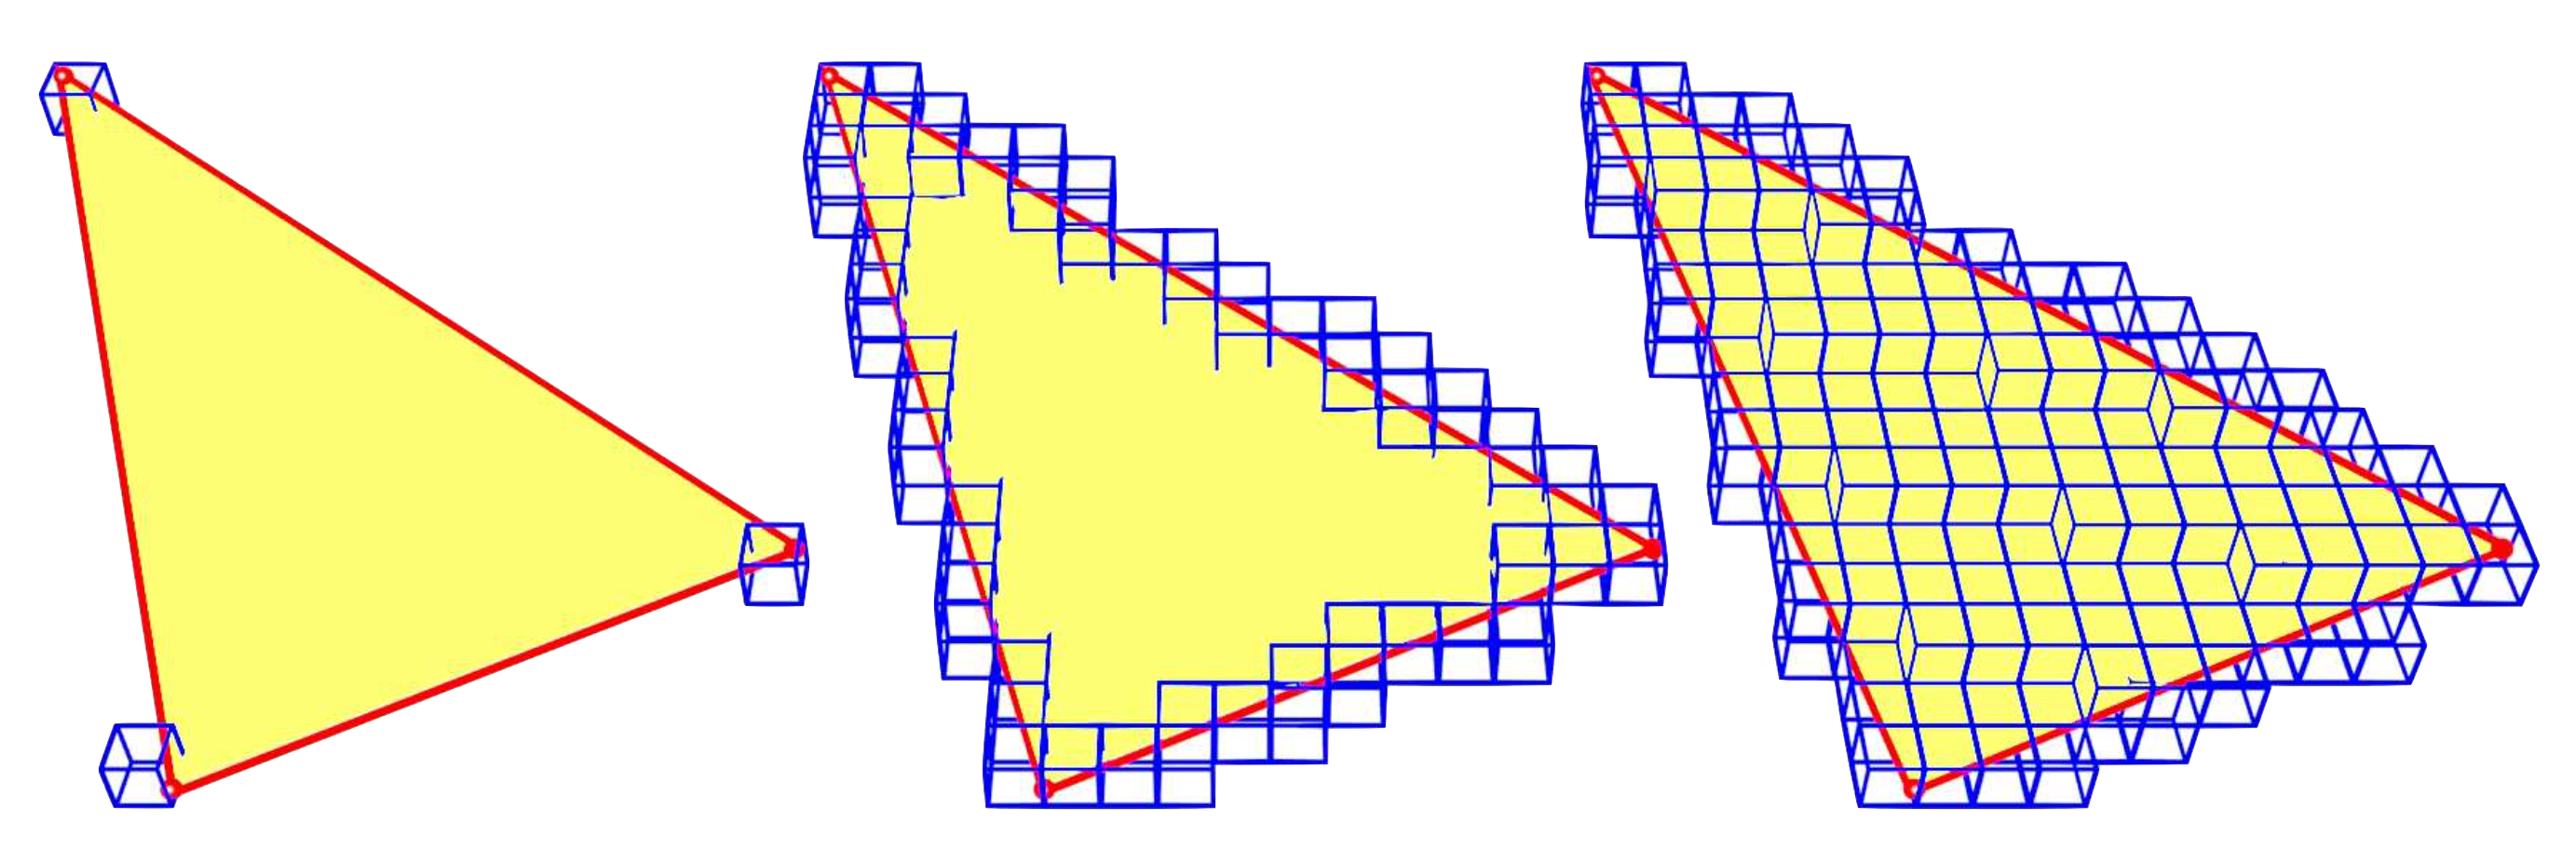
\includegraphics[width=\textwidth]{resources/voxelization_steps.png}}
      \caption*{Etapes de la voxelization}
    \end{subfigure}
    \hspace{1.2cm}
    \begin{subfigure}{0.225\textwidth}
      \frame{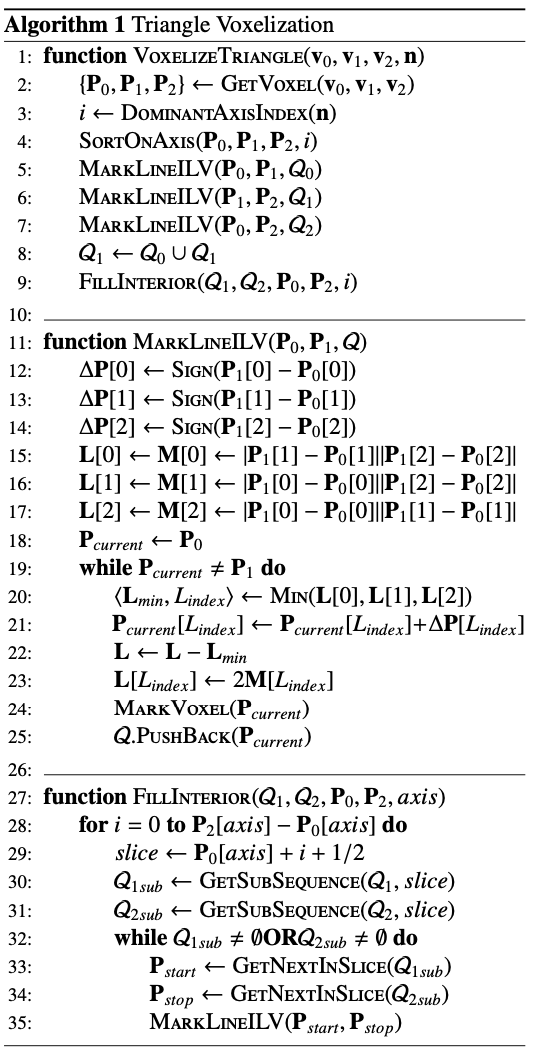
\includegraphics[width=\textwidth]{resources/algo_paper.png}}
    \end{subfigure}
  \end{figure}
\end{frame}

%--------------------------------------
\subsection{3D voxelization ? scanlines ?}

\begin{frame}[fragile=singleslide]{\insertsectionhead}
  \framesubtitle{\insertsubsectionhead}
  \begin{figure}
      \begin{subfigure}{1\textwidth}
        \frame{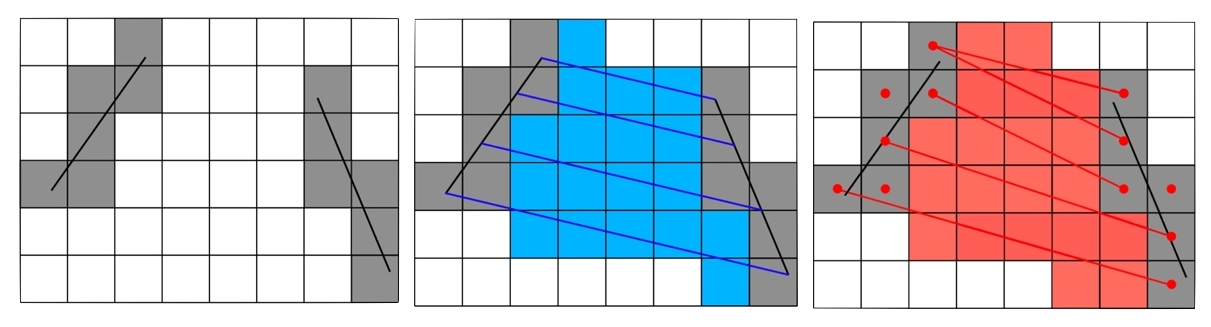
\includegraphics[width=\textwidth]{resources/scanlines.png}}
      \end{subfigure}
    \end{figure}
\end{frame}

%--------------------------------------
\subsection{Points clés}

\begin{frame}[fragile=singleslide]{\insertsectionhead}
  \framesubtitle{\insertsubsectionhead}
  \begin{itemize}
      \item Plus c'est rapide mieux c'est
      \item Parfaitement compatible avec le multithreading
      \item Plus on a de triangles plus c'est rapide
      \item L'approximation des entiers réduit les trous dans la couverture
    \end{itemize}
    \vspace{0.5cm}
    \begin{figure}
      \begin{subfigure}{1\textwidth}
        \frame{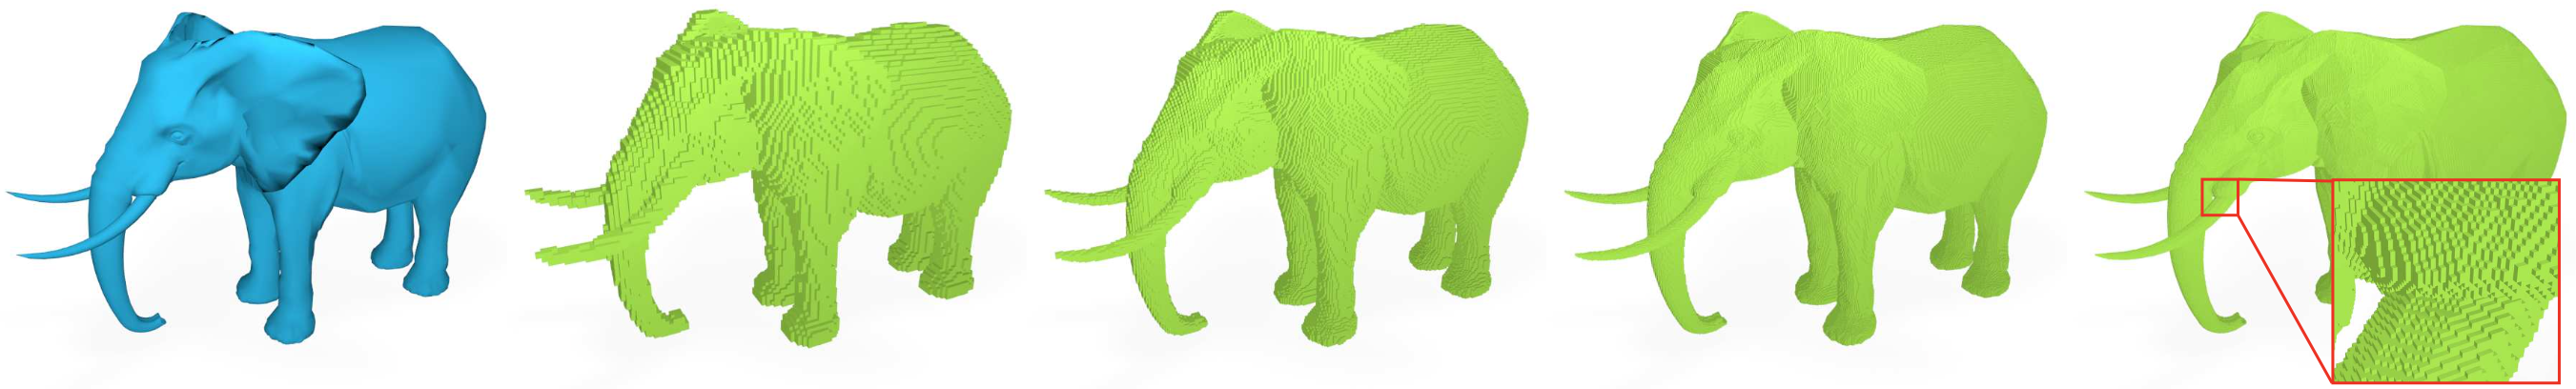
\includegraphics[width=\textwidth]{resources/elephant.png}}
      \end{subfigure}
    \end{figure}
    
    
\end{frame}

%==============================================
\section{Prototypage}
%==============================================

\subsection{Notre plan initial}

\begin{frame}[fragile=singleslide]{\insertsectionhead}
  \framesubtitle{\insertsubsectionhead}
  \begin{columns}[T,onlytextwidth]
    \column{0.4\textwidth}
      \begin{itemize}
        \item Voxelization d'un triangle
        \item Utiliser OpenGL
        \item Prototypage 2D
      \end{itemize}
    \column{0.5\textwidth}
      \begin{figure}
        \begin{subfigure}{0.4\textwidth}
          \frame{
\includegraphics[width=\textwidth]{resources/opengl_logo.png}}
        \end{subfigure}
      \end{figure}
  \end{columns}
  \vfill
  \vfill
  \hspace{0.2cm}
  {\large Nous pensions que tout était simple et clair}
\end{frame}

%--------------------------------------
\subsection{Premiers jours}

\begin{frame}[fragile=singleslide]{\insertsectionhead}
  \framesubtitle{\insertsubsectionhead}
  \begin{itemize}
    \item Reprise en main d'openGL
  \end{itemize}
  \vspace{0.3cm}
  \begin{itemize}
    \item Très satisfait du rendu du triangle à l'écran
  \end{itemize}
  \vspace{0.3cm}
  \begin{itemize}
    \item Voxelization des côtés se fait rapidement
  \end{itemize}
  \vspace{0.3cm}
  \begin{itemize}
    \item Parties qui ne sont pas claires dans l'algo
  \end{itemize}
  \vspace{0.2cm}
  \begin{figure}
        \begin{subfigure}{0.6\textwidth}
          \frame{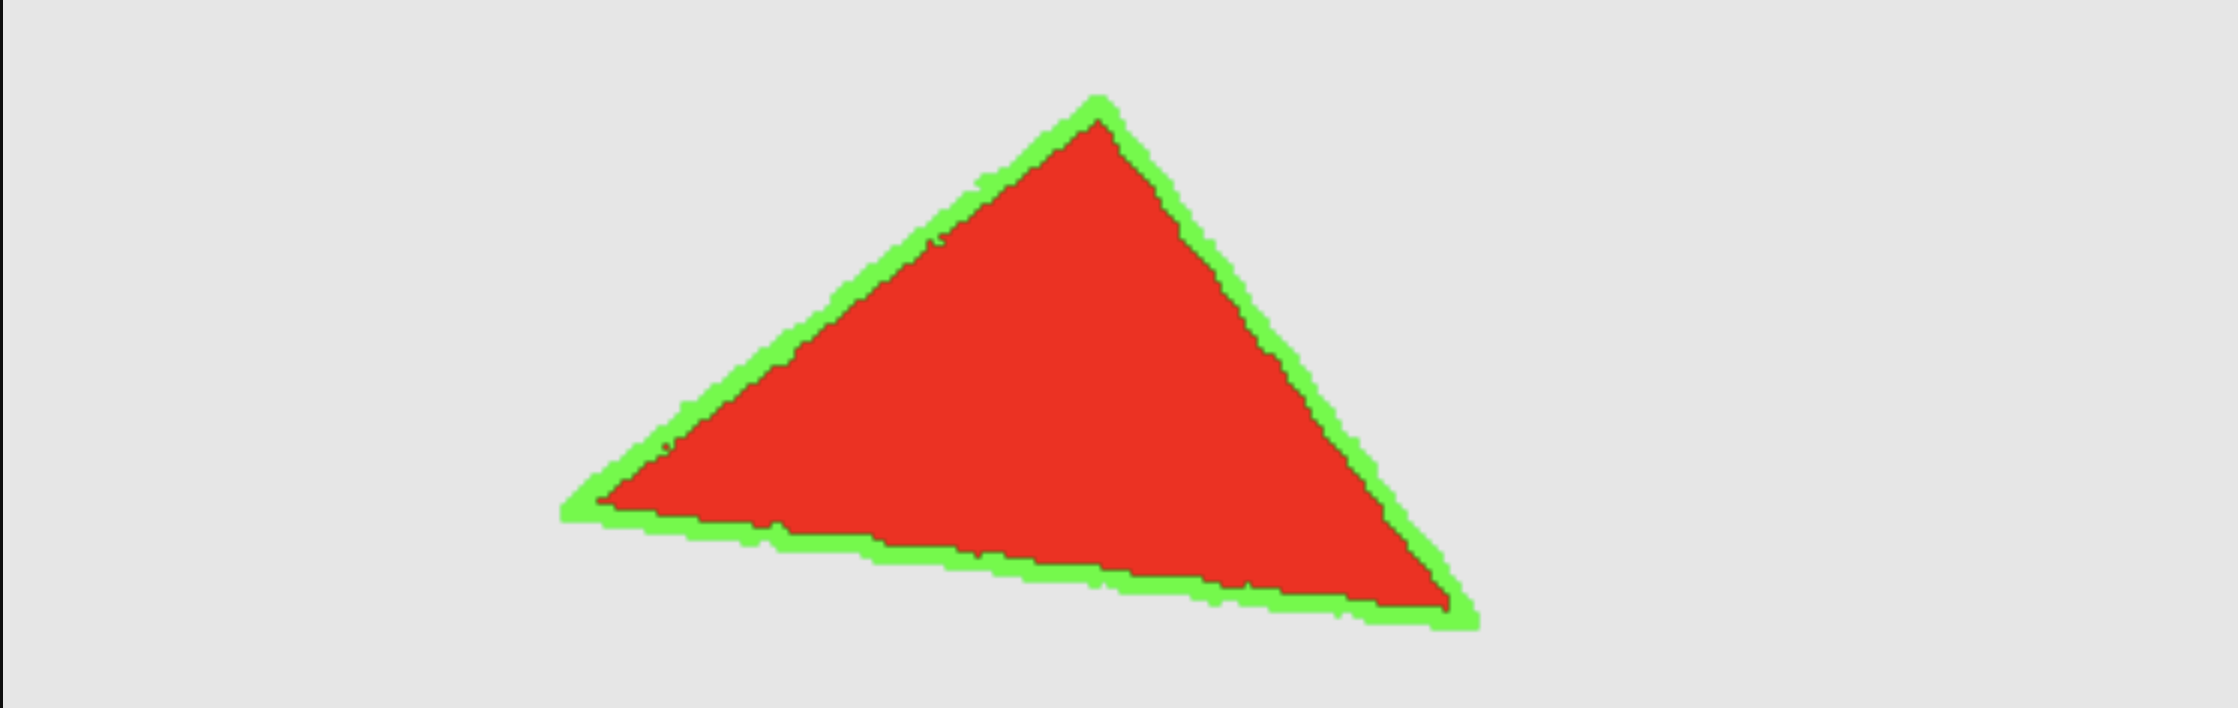
\includegraphics[width=\textwidth]{resources/voxelization_edge.png}}
          \caption*{Voxelization des côtés}
        \end{subfigure}
      \end{figure}
\end{frame}

%--------------------------------------
\subsection{Difficultés rencontrées}

\begin{frame}[fragile=singleslide]{\insertsectionhead}
  \framesubtitle{\insertsubsectionhead}
  \begin{columns}[T,onlytextwidth]
    \column{0.5\textwidth}
      \begin{itemize}
        \item Déboggage du problème de la pyramide
      \end{itemize}
      \hfill
      \begin{itemize}
        \item Essayer la méthode naïve et se rendre compte qu'elle marche mieux
      \end{itemize}
      \hfill
      \begin{itemize}
        \item Réaliser que l'algo est incomplet
      \end{itemize}
    \column{0.6\textwidth}
    \begin{figure}
        \begin{subfigure}{0.6\textwidth}
          \frame{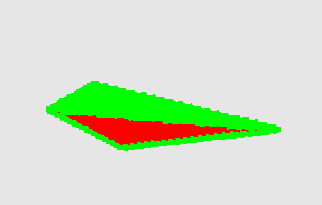
\includegraphics[width=\textwidth]{resources/pyramide_curse.png}}
        \end{subfigure}
      \end{figure}
  \end{columns}
\end{frame}

%--------------------------------------
\subsection{Éclaircissement des zones d'ombres sur l'article}

\begin{frame}[fragile=singleslide]{\insertsectionhead}
  \framesubtitle{\insertsubsectionhead}
  \begin{itemize}
    \item Relecture minutieuse de l'article pour trouver où se trouve le problème
  \end{itemize}
  \hfill
  \begin{itemize}
    \item Manque de détail dans les cas 2D
  \end{itemize}
  \hfill
  \begin{itemize}
    \item Choix d’utilisation de Bresenham dans les cas 2D
  \end{itemize}
\end{frame}

%==============================================
\section{Résultats \& Benchmark}
%==============================================

\subsection{Quelques chiffres en comparaison}

\begin{frame}[fragile=singleslide]{\insertsectionhead}
  \framesubtitle{\insertsubsectionhead}
  \begin{table}
    \centering
    \begin{tabular}{@{} lccc @{}}
      \toprule
      & \textbf{Velocity} & \textbf{Angle}  & \textbf{Vertical force} \\
      & $U$ & $\alpha$  & $F_z$ \\
      & [m/s] & [$^\circ$]  & [N] \\
      \midrule
      2D simulation  & 9 & 2 & 9.23 \\
      3D simulation  & 10.0 & 3 & 15.039 \\
      Experiment A   & 11.31 & 2.5 & 13.2 \\
      Experiment B   & 11.26 & 2.7 & 12.6 \\
      Experiment C   & 11.33 & 2.47 & 13.6 \\
      \bottomrule
    \end{tabular}
  \end{table}
\end{frame}

%--------------------------------------
\subsection{Démo}

\begin{frame}[fragile=singleslide]{\insertsectionhead}
  \framesubtitle{\insertsubsectionhead}
  \begin{figure}
    \begin{subfigure}{0.4\textwidth}
      \frame{
\includegraphics[width=\textwidth]{resources/demo.png}}
    \end{subfigure}
  \end{figure}
\end{frame}

%--------------------------------------
\subsection{Perspectives d'évolution}

\begin{frame}[fragile=singleslide]{\insertsectionhead}
  \framesubtitle{\insertsubsectionhead}
  \begin{itemize}
    \item Utiliser CUDA
  \end{itemize}
  \hfill
  \begin{itemize}
    \item Changer de langage
  \end{itemize}
  \hfill
  \begin{itemize}
    \item Passer sur du multithread
  \end{itemize}
\end{frame}

%--------------------------------------
\subsection{Conclusion}

\begin{frame}[fragile=singleslide]{\insertsectionhead}
  \framesubtitle{\insertsubsectionhead}
  {\Large Implémentation de l’algo de voxelization de l’article en OpenGL réussi mais avec notre interprétation pour le problème des cas 2D}
\end{frame}

